% Created 2025-06-07 Sat 14:57
% Intended LaTeX compiler: pdflatex
\documentclass[aspectratio=169]{beamer}
\usepackage[utf8]{inputenc}
\usepackage[T1]{fontenc}
\usepackage{graphicx}
\usepackage{longtable}
\usepackage{wrapfig}
\usepackage{rotating}
\usepackage[normalem]{ulem}
\usepackage{amsmath}
\usepackage{amssymb}
\usepackage{capt-of}
\usepackage{hyperref}
\usepackage[style=apa, backend=biber]{biblatex}
\DeclareLanguageMapping{american}{american-apa}
\addbibresource{./refs/refs.bib}
\AtEveryBibitem{\clearfield{note}}
\usepackage{endnotes}
\let\footnote=\endnote
\usepackage{./jtc}
\usetheme{default}
\author{Evan Misshula}
\date{\today}
\title{Introduction to Machine Learning Analysis and Modeling}
\hypersetup{
 pdfauthor={Evan Misshula},
 pdftitle={Introduction to Machine Learning Analysis and Modeling},
 pdfkeywords={},
 pdfsubject={},
 pdfcreator={Emacs 29.3 (Org mode 9.6.15)}, 
 pdflang={English}}
\begin{document}

\maketitle
g
\section{Ingestion \& Preprocessing}
\label{sec:org0936bd6}
\begin{frame}[label={sec:org83f0076}]{End to end process}
Recall \alert{ML workflow} is a sequence of steps to build and deploy a model that
solves a problem using data.
\end{frame}

\begin{frame}[label={sec:org60b278a}]{The pipeline}
:BEAMER\textsubscript{env}: block
:END:

\begin{center}
\begin{tabular}{llll}
Ingestion \& Preprocessing & \alert{Analysis} & Modeling & Deployment\\[0pt]
\hline
Definition & \alert{EDA} & Selection & Tuning\\[0pt]
Data Collection & \alert{Feature Engineering} & Training & Deployment\\[0pt]
Cleaning &  & Evaluation & Monitoring\\[0pt]
\end{tabular}
\end{center}
\end{frame}

\begin{frame}[label={sec:org9dd809b}]{ML Workflow Graph}
\begin{figure}[htbp]
\centering
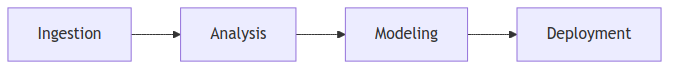
\includegraphics[width=.9\linewidth]{workflow.png}
\caption{ML workflow steps rendered as a flowchart}
\end{figure}


\begin{center}
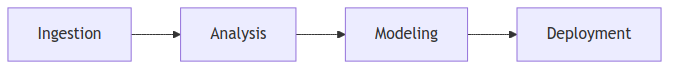
\includegraphics[width=.9\linewidth]{workflow.png}
\end{center}
\end{frame}

\section{Univariate EDA}
\label{sec:orgecb0fa2}
\begin{frame}[label={sec:orgc0eb3a7}]{Exploratory Data Analysis}
Exploratory Data Analysis (EDA) in the context of machine learning
(ML) refers to the systematic process of examining and visualizing the
structure, patterns, anomalies, and relationships within a dataset
before applying machine learning algorithms. The goal is to gain
intuition and insight about the data to inform: Understand the
distribution of each feature (e.g., normality, skewness, outliers).

Assess relationships between input features and the target variable
(e.g., correlation, mutual information).
\end{frame}


\begin{frame}[label={sec:orgaceb683},fragile]{Exploratory Data Analysis in Pandas}
 Pandas tools:
\begin{block}{`.info()` – Structure Overview}
\begin{verbatim}
df.info()
\end{verbatim}

\begin{itemize}
\item Displays a concise summary of the DataFrame:
\begin{itemize}
\item Number of non-null values per column
\item Data types of each column
\item Memory usage
\item Total number of rows and columns
\end{itemize}
\end{itemize}
\end{block}

\begin{block}{Pandas example}
\begin{verbatim}
<class 'pandas.core.frame.DataFrame'>
RangeIndex: 1000 entries, 0 to 999
Data columns (total 5 columns):
 #   Column    Non-Null Count  Dtype  
---  ------    --------------  -----  
 0   name      1000 non-null   object 
 1   age       950 non-null    float64
 2   income    1000 non-null   float64
 3   city      1000 non-null   object 
 4   joined    995 non-null    datetime64[ns]
dtypes: datetime64 , float64(2), object(2)
memory usage: 39.2+ KB
\end{verbatim}
\end{block}
\end{frame}
\begin{frame}[label={sec:org2aab128},fragile]{Pandas `.describe()`}
 \begin{block}{`.describe()` – Summary Statistics}
\begin{verbatim}
df.describe()
\end{verbatim}

\begin{itemize}
\item Returns summary statistics for numeric columns:
\begin{itemize}
\item `count`, `mean`, `std`, `min`, `25\%`, `50\%`, `75\%`, `max`
\end{itemize}
\end{itemize}

\begin{verbatim}
              age      income
count   950.000000  1000.000000
mean     35.5       60000.0
std      10.0       15000.0
min      18.0       20000.0
25%      28.0       50000.0
50%      35.0       60000.0
75%      42.0       70000.0
max      65.0       120000.0
\end{verbatim}
\end{block}
\end{frame}
\begin{frame}[label={sec:orgeb9e608},fragile]{Non-numeric results}
 For non-numeric columns:

\begin{verbatim}
df.describe(include='object')
\end{verbatim}

\begin{itemize}
\item Shows: `count`, `unique`, `top`, `freq`
\end{itemize}
\end{frame}

\begin{frame}[label={sec:org2dd0eaf}]{Pandas Tool Summary}
\begin{center}
\begin{tabular}{lll}
Method & Purpose & Applies To\\[0pt]
\hline
`df.info()` & Structure \& metadata & All columns\\[0pt]
`df.describe()` & Descriptive stats (summary) & Numeric by default\\[0pt]
\end{tabular}
\end{center}
\end{frame}

\begin{frame}[label={sec:org9475f8e}]{Univariate analysis Visualize}
\begin{block}{\alert{Look at your data}}
\begin{itemize}
\item Histogram + KDE \(\rightarrow\) quick skew/kurtosis check.
\item Q-Q Plot \(\rightarrow\) best for tail behavior.
\item Boxplot \(\rightarrow\) highlights symmetry and outliers.
\end{itemize}
[Live Code 2]
\end{block}
\end{frame}

\begin{frame}[label={sec:orgd86562f}]{Univariate Analysis Tests}
\begin{block}{Tests for Skewness and Kurtosis}
\begin{itemize}
\item \alert{D'Agostino's \(K^2\) Test}: Combines measures of skewness and kurtosis.
\begin{itemize}
\item Based on transformations of the sample skewness and kurtosis.
\item Null Hypothesis: The data is normally distributed.
\item Available in `scipy.stats.normaltest`.
\end{itemize}
\begin{itemize}
\item \alert{\alert{Jarque–Bera Test}}:
\begin{itemize}
\item Specifically evaluates skewness and excess kurtosis against a normal distribution.
\item Null Hypothesis: Data is normally distributed.
\end{itemize}
\end{itemize}
\end{itemize}
\end{block}
\end{frame}

\begin{frame}[label={sec:org9b4c846}]{Summary Univariate Analysis}
\begin{block}{Interpretation}
\begin{itemize}
\item \alert{Low p-value (< 0.05)}: Reject null \(\rightarrow\) evidence of
non-normal skew/kurtosis.
\item \alert{High p-value (≥ 0.05)}: Fail to reject null \(\rightarrow\) no
evidence of non-normality.
\end{itemize}
\end{block}
\end{frame}

\section{Multivariate EDA}
\label{sec:orgdb4f9c1}
\begin{frame}[label={sec:org379917c}]{Motivation for Multivariate EDA}
\begin{itemize}
\item Univariate EDA is insufficient for understanding dependencies and
structure in multivariate data.
\item Multivariate EDA focuses on relationships, redundancy, and
conditional structure across features.
\item Goal: Identify informative, redundant, or interacting features.
\end{itemize}
\end{frame}

\begin{frame}[label={sec:org6e473b8}]{Joint and Marginal Distributions}
\begin{itemize}
\item Let \(X = (X_1, X_2, \ldots, X_d) \in \mathbb{R}^d\) be a random
vector.
\item The \alert{joint distribution} \(P_X\) describes full probabilistic
structure.
\item The \alert{marginal distribution} of a feature \(X_i\) is obtained by
integrating out all other variables.
\item Understanding joint vs. marginal behavior is central to multivariate
EDA.
\end{itemize}
\end{frame}

\begin{frame}[label={sec:org5e2b87c}]{Statistical Dependence}
\begin{itemize}
\item Two variables \(X\) and \(Y\) are independent if:
\[
  P_{X,Y}(x, y) = P_X(x) P_Y(y)
  \]
\item EDA seeks to \alert{discover} dependencies between variables.
\item Classical tools: covariance, correlation — but these are limited to
linear dependence.
\end{itemize}
\end{frame}

\begin{frame}[label={sec:org3affee5}]{Mutual Information}
\begin{itemize}
\item Mutual Information (MI) is a nonparametric measure of dependence:
\[
  I(X; Y) = \int \int p(x,y) \log \left( \frac{p(x,y)}{p(x)p(y)} \right) dx dy
  \]
\item \(I(X;Y) = 0\) iff \(X \perp Y\).
\item Captures all kinds of dependence — not just linear.
\end{itemize}
\end{frame}

\begin{frame}[label={sec:orgc6385ee}]{Connection to KL Divergence}
\begin{itemize}
\item Mutual Information is a special case of the \alert{Kullback-Leibler
divergence}:
\[
  I(X;Y) = D_{\mathrm{KL}}(P_{X,Y} \| P_X \otimes P_Y)
  \]
\item It measures how far the joint distribution is from the product of the marginals.
\item Interpreted as: \alert{How surprising is the joint distribution, compared to independence?}
\end{itemize}
\end{frame}

\begin{frame}[label={sec:org5d05c36}]{Why It Matters in EDA}
\begin{itemize}
\item Helps detect feature redundancy or relevance.
\item Basis for feature selection and structure learning.
\item Multivariate visualizations (pair plots, heatmaps, etc.) are
motivated by mathematical notions of dependence.
\end{itemize}
[Live Code]
\end{frame}
\section{KL Divergence}
\label{sec:org4aa8cb0}
\begin{frame}[label={sec:org71dac23}]{What is KL Divergence?}
KL Divergence is a measure of how one probability distribution \(Q\) differs from a reference distribution \(P\).

\begin{itemize}
\item It is not symmetric: \(D_{KL}(P \parallel Q) \neq D_{KL}(Q \parallel P)\)
\item KL divergence is always non-negative: \(D_{KL}(P \parallel Q) \geq 0\)
\item \(D_{KL}(P \parallel Q) = 0\) if and only if \(P = Q\) almost everywhere
\end{itemize}
\end{frame}

\begin{frame}[label={sec:orgaecf1f5}]{Mathematical Definition (Discrete)}
Let \(P\) and \(Q\) be probability mass functions over a finite or countable set \(\mathcal{X}\).

\begin{equation}
D_{KL}(P \parallel Q) = \sum_{x \in \mathcal{X}} P(x) \log \frac{P(x)}{Q(x)}
\end{equation}

\begin{itemize}
\item The log is typically taken to base 2 (bits) or base \(e\) (nats)
\item Requires \(Q(x) > 0\) wherever \(P(x) > 0\)
\end{itemize}
\end{frame}

\begin{frame}[label={sec:orgb112d85}]{Interpretation}
\begin{itemize}
\item Measures the expected number of \alert{extra bits} needed to code samples
from \(P\) using a code optimized for \(Q\)
\item It is the \alert{relative entropy} of \(P\) with respect to \(Q\)
\end{itemize}
\end{frame}

\begin{frame}[label={sec:org26b62cf}]{Mathematical Definition (Continuous)}
Let \(p(x)\) and \(q(x)\) be probability density functions over a
domain \(\mathcal{X} \subseteq \mathbb{R}^n\):

\begin{equation}
D_{KL}(P \parallel Q) = \int_{\mathcal{X}} p(x) \log \frac{p(x)}{q(x)} \, dx
\end{equation}

\begin{itemize}
\item Again, the divergence is zero iff \(p(x) = q(x)\) almost everywhere
\end{itemize}
\end{frame}

\begin{frame}[label={sec:orge710ba3}]{Practical Calculation}
Given empirical data samples \(x_1, \dots, x_n \sim P\), estimate KL divergence:

\begin{itemize}
\item Use histograms or kernel density estimators (KDE) to estimate \(p(x)\), \(q(x)\)
\item Approximate:
\end{itemize}

\begin{equation}
\hat{D}_{KL}(P \parallel Q) = \frac{1}{n} \sum_{i=1}^n \log \frac{p(x_i)}{q(x_i)}
\end{equation}

\begin{itemize}
\item Common in variational inference and mutual information estimation
\end{itemize}
\end{frame}

\begin{frame}[label={sec:org5039c5c}]{KL Divergence vs. Other Measures}
\begin{center}
\begin{tabular}{lll}
Measure & Symmetric & Interpretable\\[0pt]
\hline
KL Divergence & ✗ & Code inefficiency\\[0pt]
Jensen-Shannon & ✓ & Interpolated KL\\[0pt]
Mutual Information & ✓ & Redundancy\\[0pt]
\end{tabular}
\end{center}
\end{frame}

\begin{frame}[label={sec:org20c2393}]{Summary of KL Divergence}
\begin{itemize}
\item KL divergence quantifies divergence from a reference distribution
\item Central to many ML methods: variational inference, GANs, language modeling
\item Not symmetric, not a true metric
\item Requires careful estimation for continuous variables
\end{itemize}
\end{frame}

\section{Feature Engineering}
\label{sec:orgc50ecb3}

\begin{frame}[label={sec:org932f06c}]{What is Feature Engineering?}
\begin{itemize}
\item Feature engineering is the process of transforming raw data into
meaningful input features for machine learning models.
\item It involves:
\begin{itemize}
\item Creating new features
\item Modifying existing ones
\item Selecting the most relevant subset
\end{itemize}
\item The goal is to enhance model performance by exposing the most useful signal in the data.
\end{itemize}
\end{frame}

\begin{frame}[label={sec:org166b277}]{Why is Feature Engineering Important?}
\begin{itemize}
\item Quality of features often outweighs choice of algorithm.
\item Poor features = poor model performance, regardless of the model used.
\item Good features can:
\begin{itemize}
\item Improve accuracy
\item Speed up training
\item Reduce overfitting
\item Make models interpretable
\end{itemize}
\end{itemize}
\end{frame}

\begin{frame}[label={sec:orgbcf3af6}]{Common Types of Feature Engineering}
\begin{itemize}
\item \alert{Normalization/Scaling}: StandardScaler, MinMaxScaler
\item \alert{Encoding}: One-hot, Label encoding
\item \alert{Discretization/Binning}
\item \alert{Polynomial Features}: Capture interactions
\item \alert{Date/Time decomposition}: Day, month, weekday, etc.
\item \alert{Log transformations}: For skewed distributions
\end{itemize}
\end{frame}

\begin{frame}[label={sec:org5851767}]{Feature Selection and Extraction}
\begin{itemize}
\item \alert{Feature Selection}: Identify and keep the most relevant variables.
\begin{itemize}
\item \alert{RFE (Recursive Feature Elimination)}:
\begin{itemize}
\item Iteratively builds a model and removes the least important feature.
\item Works with any estimator that exposes `coef\_` or `feature\textsubscript{importances}\_`.
\end{itemize}
\end{itemize}
\item \alert{Feature Extraction}: Derive new features from raw data.
\begin{itemize}
\item \alert{t-SNE (t-distributed Stochastic Neighbor Embedding)}:
\begin{itemize}
\item A nonlinear dimensionality reduction technique.
\item Preserves local structure; useful for visualizing high-dimensional data.
\end{itemize}
\item \alert{UMAP (Uniform Manifold Approximation and Projection)}:
\begin{itemize}
\item Similar to t-SNE but faster and better preserves global structure.
\item Based on topological and geometric foundations.
\end{itemize}
\end{itemize}
\end{itemize}
\end{frame}

\begin{frame}[label={sec:org8a8e006}]{Best Practices and Guidelines}
\begin{itemize}
\item Understand the data context and business goals.
\item Visualize feature distributions and relationships.
\item Watch out for data leakage.
\item Use cross-validation to evaluate engineered features.
\end{itemize}
\end{frame}

\begin{frame}[label={sec:org2686c5c}]{Summary of Feature Engineering}
\begin{itemize}
\item Feature engineering is essential for successful modeling.
\item Methods like RFE, t-SNE, and UMAP help in selection and dimensionality reduction.
\item Combining domain knowledge with statistics is key.
\end{itemize}
\end{frame}
\end{document}
